\section{Results}
\subsection{Self-play converges to stable task-level equilibria}
The first question is whether mission-level self-play produces a reproducible endpoint rather than a transient training phase. Figure~\ref{fig:training} shows the full three-stage trajectory for S7 seed 20260801.
\begin{figure}[t]
\centering
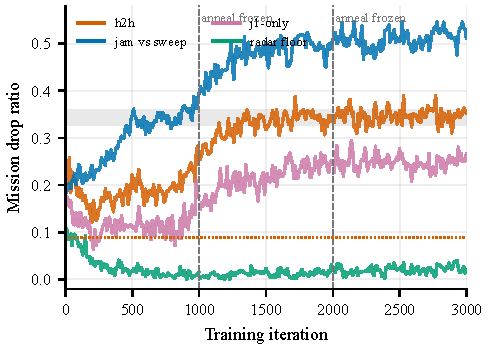
\includegraphics[width=\columnwidth]{figures/fig2_training_curves.pdf}
\caption{Three-stage S7 trajectory for seed 20260801. Dashed lines mark the 1000- and 2000-iteration continuation boundaries; the final region is stationary across the four evaluation views.}
\label{fig:training}
\end{figure} After the entropy schedule was frozen, the five 200-iteration windows from 2000 to 3000 had h2h means 0.3465, 0.3428, 0.3484, 0.3507, and 0.3463. The corresponding jam-vs-sweep means were 0.5121, 0.4956, 0.5118, 0.5107, and 0.5215. This continuation therefore rules out both an early stopping artifact and a persistent drift. The last 40 validation points at 3000 give h2h $0.3485\pm0.0151$ and jam-vs-sweep $0.5161\pm0.0174$.

The same endpoint appears across three converged S7 seeds. Full-protocol evaluation gives h2h drops of 0.3390, 0.3212, and 0.3496, with an across-seed mean of $0.3366\pm0.0143$. The idle-radar drop is $0.0194\pm0.0008$ in S7, compared with $0.0242\pm0.0097$ across the three valid S6 seeds; both values remain low. The convergence result is descriptive: it establishes a stable attractor for this benchmark and training protocol, not a proof of global Nash equilibrium.

A response-set exploitability measure sharpens what stationarity does and does not imply. We evaluate each team against every alternative response in our evaluation set and sum the best deviation gains, an upper-bound-free, response-set-restricted analog of NashConv. The jammer team has no improving deviation in the set: the trained pair's drop of $0.3366$ exceeds the singleton ($0.2086\pm0.0745$), the stare pair ($0.2374\pm0.0036$), and the random pair ($0.0922\pm0.0047$) against the same radars. The radar team does: deviating to the greedy mission-stare policy recovers $0.3366-0.0889=0.2477$ of drop against the same jammers. The response-set exploitability of the converged pair is therefore $0.2477$, driven entirely by the radar side. We report this as a lower bound over an enumerated response set, not exact exploitability: it quantifies that the stationarity of Fig.~\ref{fig:training} reflects mutual co-adaptation within the training distribution, while a measurable exploit remains available to out-of-distribution responses---the phenomenon that Sections~V-C and V-D develop.

The containment result also survives a change of learning rule. An IPPO control---four independent PPO learners, no parameter sharing, no centralized critic, everything else bit-identical---reaches the same 2000-iteration protocol point at h2h $0.2472$, jam-vs-sweep $0.4123$, and neutralization $23.3\%$, versus $0.3282$, $0.5043$, and $20.2\%$ for MAPPO at the same budget. Absolute levels differ on both sides, but the floor-adjusted containment ratio barely moves: the attacker-count effect is a property of the game's structure, not of MAPPO's centralized critic, and $\eta$ itself is robust to the learner's strength.

\subsection{Doubling the attacker reduces defense containment by two-thirds}
The main comparison is summarized in Table~\ref{tab:main} and Figure~\ref{fig:neutralization}.
\begin{figure}[t]
\centering
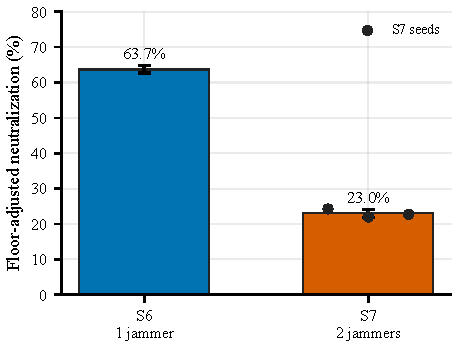
\includegraphics[width=\columnwidth]{figures/fig3_neutralization.pdf}
\caption{Floor-adjusted neutralization for the S6 and S7 games. The dots show the three converged S7 training seeds; error bars are standard deviations across training seeds (S6 uses the three valid 12-dB seeds).}
\label{fig:neutralization}
\end{figure} In S6, the valid three-seed 12-dB h2h drop is $0.0860\pm0.0061$, jam-vs-sweep is $0.2727\pm0.0088$, and floor-adjusted neutralization is $62.8\%\pm1.6\%$. In converged S7, these values become $0.3366\pm0.0143$, $0.5294\pm0.0215$, and $23.0\%\pm1.1\%$, respectively.

The neutralization change is not a consequence of a corresponding radar collapse. Learned radars facing idle jammers retain a low drop of $0.0194\pm0.0008$ in S7, compared with $0.0242\pm0.0097$ across the three valid S6 seeds. Instead, two jammers increase the marginal disruption that survives radar adaptation. The jammer team's raw disruption against scripted sweeps rises by 94\% relative to S6, while the fraction of that disruption removed by learned radars falls by approximately two-thirds. Because the comparison controls total jammer activation but also changes radar-site geometry, this is a benchmark-level scaling result rather than a fully isolated attacker-count intervention.

\begin{table}[t]
\caption{Converged S6--S7 comparison. Drop is the mission-loss ratio; $\eta$ is floor-adjusted defense neutralization.}
\label{tab:main}
\centering
\small
\begin{tabular}{lcc}
\toprule
Metric & S6: 1v2 & S7: 2v2 \\
\midrule
h2h drop & $0.0860\pm0.0061$ & $0.3366\pm0.0143$ \\
jam-vs-sweep drop & $0.2727\pm0.0088$ & $0.5294\pm0.0215$ \\
rad-vs-idle drop & $0.0242\pm0.0097$ & $0.0194\pm0.0008$ \\
$\eta$ & $62.8\%\pm1.6\%$ & $23.0\%\pm1.1\%$ \\
\bottomrule
\end{tabular}
\end{table}

\subsection{Scripted baselines anchor both teams and expose co-adaptation}
Table~\ref{tab:baselines} evaluates the converged teams against four scripted policies under the identical 64-scenario, three-action-seed protocol. Both learned teams dominate their non-learning counterparts: a random legal radar loses $0.5085\pm0.0051$ of missions against the trained jammer pairs versus $0.3366\pm0.0143$ for the trained radar team, and random or stare jammers impose only $0.0922\pm0.0047$ and $0.2374\pm0.0036$ against the trained radars versus $0.3366\pm0.0143$ for the trained jammer pairs. Learning is real on both sides of the link.

\begin{table}[t]
\caption{Evaluation-only scripted baselines against the converged S7 teams (mission drop; mean $\pm$ sd across three training seeds, three action seeds each). EDF is a deadline-informed oracle (privileged deadline state).}
\label{tab:baselines}
\centering
\small
\begin{tabular}{lc}
\toprule
Policy & Mission drop \\
\midrule
\multicolumn{2}{l}{\emph{Radar side, vs.\ trained jammer pairs}} \\
Learned radar team (h2h) & $0.3366\pm0.0143$ \\
Scripted sweep & $0.5294\pm0.0215$ \\
Random legal radar & $0.5085\pm0.0051$ \\
Greedy mission-stare radar & $0.0889\pm0.0000$ \\
EDF oracle radar & $0.2961\pm0.0039$ \\
\midrule
\multicolumn{2}{l}{\emph{Jammer side, vs.\ trained radar teams}} \\
Learned jammer pair (h2h) & $0.3366\pm0.0143$ \\
Stare jammer pair & $0.2374\pm0.0036$ \\
Random legal jammer pair & $0.0922\pm0.0047$ \\
Idle jammers (reference) & $0.0194\pm0.0008$ \\
\bottomrule
\end{tabular}
\end{table}

The greedy mission-stare radar is the informative exception. Pointing both heads at the heaviest pending service--azimuth cell yields a drop of exactly $0.0889$ against every trained jammer pair and every action seed---a factor of 3.8 below the learned h2h drop and below even the natural scheduling floor of $0.1187$ (sweep radars facing idle jammers). The zero variance is not an evaluation artifact: the greedy policy is deterministic given the observations, and none of the jammer action streams sampled across nine (team, action-seed) combinations flips any per-step detection outcome under the stare margin, so mission completion is fully determined by the arrival and scheduling process. (Its three-decimal coincidence with the S6 h2h value 0.0888 is chance; the two numbers come from independent evaluation pipelines over different games.) Under this link budget, the pointing gain at the exact mission bearing creates a detection margin that none of the three trained jammer teams overcomes: their learned advantage applies to radars that spread attention (sweeps, $0.5294$; the learned equilibrium radar, $0.3366$), not to a well-pointed stare. The ordering among heuristics is itself diagnostic: the hottest-queue stare ($0.0889$) dominates a deadline-first oracle ($0.2961\pm0.0039$) despite the latter's privileged deadline access, because per-step detection is probabilistic and grinding the densest pending sector converts more expected detections than chasing the single earliest deadline.

This reframes the h2h value and $\eta$: they are equilibrium quantities, not radar performance ceilings. The self-play radar hedges against its co-trained opponent at the cost of mission throughput, and the learned jammer team is exploitable by an out-of-distribution non-learning policy---the radar-side counterpart of the singleton result in Section~V-D. A jammer team co-trained against greedy radars would plausibly restore the penalty; testing that counter-adaptation requires new training runs and is left as future work.

\subsection{When does pointing discipline dominate?}
The stare result can be decomposed analytically. Holding the jammer allocation fixed and varying only the radar beam, exact mission-bearing pointing weakly dominates the neighboring beam at \emph{every} azimuth and \emph{every} jammer power we tested (0.1--12.8 W per cell): the pointing-gain term always exceeds the exposure penalty, so per-step detection satisfies $p_{\mathrm{exact}}\ge p_{\mathrm{off}}$ by construction of the link budget. Within a deadline window of at most six steps, the success probabilities compound as $1-(1-p)^{6}$, so even a factor-of-two per-step advantage compounds into an overwhelming window advantage. Pointing discipline is therefore always weakly optimal per target; the residual scheduling question is \emph{which} mission to point at when several contend, which is where the heuristic ordering of Table~\ref{tab:baselines} comes from. The hottest-queue rule concentrates both heads on the densest pending sector, converting each step into two independent detection trials on the same mission; the EDF oracle instead chases the single earliest deadline, spreading the same looks across sectors and paying the off-bearing pointing loss on most of them. Under stochastic per-step detection, concentrating looks on the densest sector maximizes expected completions per step, which is why the oracle's privileged deadline knowledge buys less than queue density.

The absolute survival level, however, is strategic rather than physical. We recomputed the stare window success under a worst-case aimed jammer pair (both jammers choosing the received-power-maximizing beam against the stared radar, one cell each, the deployed per-step activation): the six-step success probability collapses to between 0.004 and 0.317 depending on azimuth, versus near-unity under the fixed benign allocation used in the pre-training gate (Fig.~\ref{fig:benchmark}). The trained jammer teams play mixed beam policies between these two bounds, and the observed greedy-stare success of $0.911$ lies in that interval. A budget-concentration scan sharpens the boundary: stacking 2 cells in a single aimed step already reduces the worst-azimuth stare window success below $10^{-3}$. The stare margin that the trained teams leave on the table is thus a property of their learned allocation, not of the physics---precisely the question the counter-adaptation control (jammers trained against a fixed stare radar) is designed to answer.

\subsection{Attacker count is primary; cross-fire geometry is secondary}
The co-located-jammer control tests whether the S7 result requires two spatially separated jammers. It places both jammer sites at $+60^\circ$ while retaining the two radar sites at $\pm20^\circ$, the same physics, budget, two-stage training, and final evaluation, replicated across three training seeds. The control yields h2h $0.3033\pm0.0102$, jam-vs-sweep $0.4978\pm0.0081$, and neutralization $26.6\%\pm2.9\%$ (per-seed $28.4\%$, $23.2\%$, $28.1\%$).

Thus, the matched S7 geometry control shows that two jammers account for most of the containment loss within the separated-radar setting: containment is $26.6\%\pm2.9\%$ for co-located jammers and $24.2\%$ for cross-fire. The S6-to-S7 comparison additionally changes radar-site geometry, so the full count effect is a benchmark-level attribution rather than a perfectly isolated causal contrast. The cross-fire comparison itself is controlled for radar placement, budget, training protocol, and evaluation. The pre-specified contestability profiles and the matched control are shown in Figure~\ref{fig:benchmark}; the converged mechanism decomposition is shown in Figure~\ref{fig:ablation}.
\begin{figure*}[t]
\centering
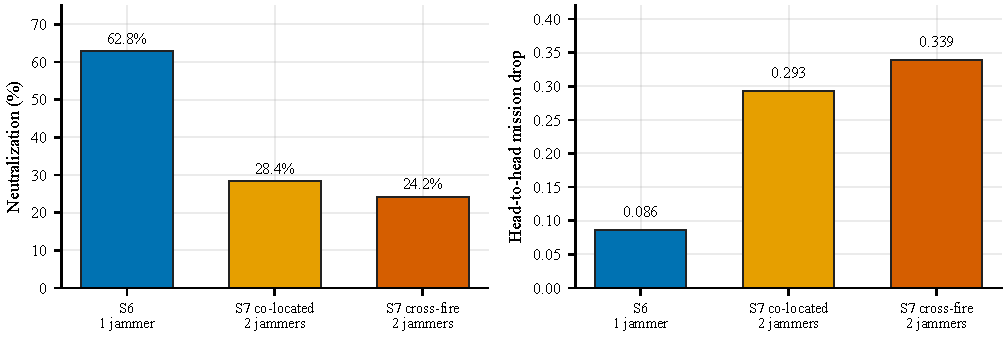
\includegraphics[width=0.96\textwidth]{figures/fig4_mechanism_ablation.pdf}
\caption{Mechanism decomposition under matched task, budget, and training protocols. Two co-located jammers reproduce most of the containment loss, while cross-fire geometry adds a secondary penalty.}
\label{fig:ablation}
\end{figure*}

\subsection{Containment saturates beyond two attackers at fixed budget}
The attacker-count axis extends beyond the matched control by training the n-jammer game at $n=3$ (sites $+60^\circ, 0^\circ, -60^\circ$, budget split 21/21/21) under the identical two-stage protocol, with the $n=2$ cross-fire run as the reference. Pre-training gate profiles computed with the exact published semantics reproduce the $n=2$ profile digit-for-digit and pass for the arc placement, so the extension stayed inside the validated regime. Across three converged $n=3$ seeds, neutralization is $22.2\%\pm1.5\%$ (h2h $0.224$, jam-vs-sweep $0.362$)---statistically indistinguishable from the $n=2$ value of $24.2\%$, while the raw disruption against scripted sweeps \emph{falls} from $0.529$ to $0.362$.

The scaling picture is therefore not monotone in attacker count at fixed total budget: the containment break occurs at the $1\to2$ step ($62.8\%$ to mid-20s), and adding a third jammer neither deepens it nor further erodes containment. The per-jammer budget, not the count, becomes the binding variable---21 tokens per jammer dilute each site's peak disruptive power below what the pairwise equilibrium extracts from 31--32 tokens. For defense design this is the useful direction of the result: the stress test that matters is the transition from one source to two, and beyond that the antagonist's total energy budget dominates its distribution across platforms.

\subsection{Counter-adaptation: the stare margin is learnable to attack}
The greedy-stare result of Section~V-C leaves open whether a jammer team \emph{could} punish the stare or merely had not. The counter-adaptation control answers it: training the jammer team against a fixed greedy-stare radar (radar updates skipped) drives the stare's drop from the static $0.0889$ to $0.213$ by iteration 2000---a factor of 2.4, still trending upward at the end of the run. Three consequences follow. The zero-variance baseline was not an evaluation artifact: a co-trained opponent moves it. The margin is strategic rather than physical, exactly as the worst-case-aimed analysis of Section~V-C predicted (the aimed bound sits at $0.68$--$1.00$ drop). And plain self-play simply never visited the stare in its opponent distribution---the same specialization failure that Section~V-D exposed on the radar side, now demonstrated on the jammer side under training.

\subsection{Pair-trained defenses trade singleton robustness for pairwise defense}
The fourth view evaluates one learned jammer against radars trained in the 2v2 game. Across the three converged S7 seeds, the singleton drop is 0.2632, 0.2387, and 0.1238, with mean $0.2086\pm0.0745$. This variation is larger than the h2h variation, but all three seeds expose the same opponent-class boundary: a defense optimized against a pair is not uniformly robust to a singleton. The spread itself is mechanistically plausible---the pair-trained radar heads divide the azimuth plane between sectors, and how well that division happens to cover the surviving jammer's bearing varies per seed---and the per-seed behavior extractions in the artifact allow this attribution to be checked directly.

The seed-01 continuation makes the trade-off visible over time. As the pair-trained equilibrium develops, j1-only rises from approximately 0.12 near the 1000-iteration checkpoint to approximately 0.24 at 2000 and remains near 0.25 at 3000, while h2h settles near 0.34. Radar competence against idle jammers remains low and stable. The result is therefore an adaptation trade-off, not evidence that the radar actor or critic stopped learning.

The learned behavior is interpretable and is summarized in Figure~\ref{fig:behavior}.
\begin{figure*}[t]
\centering
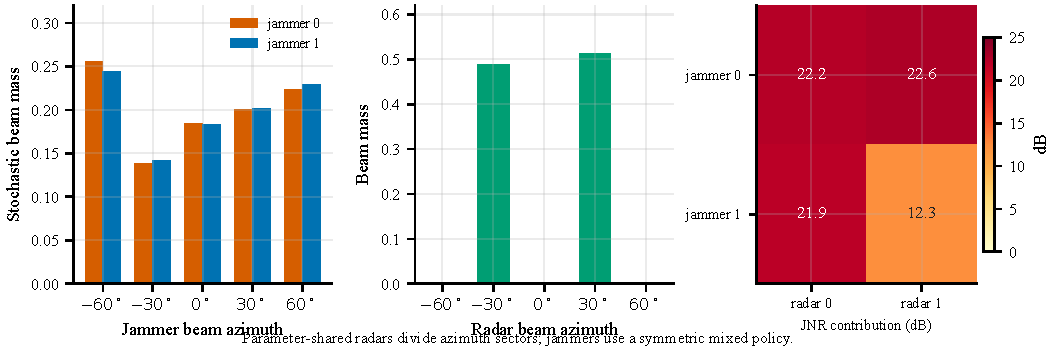
\includegraphics[width=0.96\textwidth]{figures/fig5_behavior.pdf}
\caption{Equilibrium behavior at the converged S7 checkpoint. Radar heads divide the mission plane between two azimuth sectors, while the jammer team uses a symmetric mixed beam policy. The heat map reports active-only pairwise JNR contributions in dB.}
\label{fig:behavior}
\end{figure*}

\subsection{Opponent-class mixing reduces singleton leverage}
The full dose-response is shown in Figure~\ref{fig:r5} and Table~\ref{tab:r5}.
\begin{figure}[t]
\centering
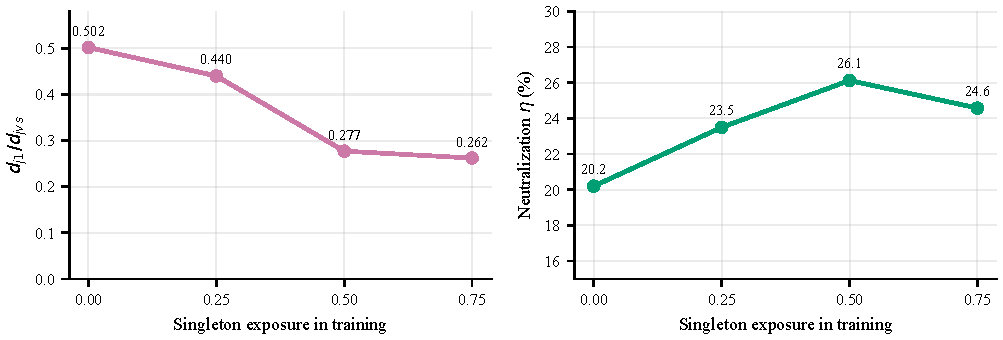
\includegraphics[width=\columnwidth]{figures/fig6_r5_dose_response.pdf}
\caption{R5-lite opponent-class mixing. Singleton relative leverage $d_{j1}/d_{jvs}$ falls with singleton exposure, while floor-adjusted neutralization peaks near 50\%. Absolute drops are confounded by skipped jammer updates.}
\label{fig:r5}
\end{figure}
\begin{table}[t]
\caption{R5-lite opponent-class mixture. Absolute drops are descriptive because singleton iterations skip the jammer update; ratio metrics are the primary comparison.}
\label{tab:r5}
\centering
\small
\begin{tabular}{lccccc}
\toprule
$q$ & h2h & jvs & j1-only & j1/jvs & $\eta$ \\
\midrule
0 & .3282 & .5043 & .2532 & .502 & 20.2\% \\
.25 & .2470 & .4015 & .1767 & .440 & 23.5\% \\
.50 & .1962 & .3580 & .0992 & .277 & 26.1\% \\
.75 & .1939 & .3476 & .0911 & .262 & 24.6\% \\
\bottomrule
\end{tabular}
\end{table}

Singleton relative leverage $d_{\mathrm{j1}}/d_{\mathrm{jvs}}$ falls monotonically from 0.502 to 0.262 and saturates between 50\% and 75\% exposure. The containment ratio $\eta$ increases from 20.2\% to 26.1\% at 50\% exposure before leveling at 24.6\%. The h2h-to-jvs ratio is $0.651$ at $q=0$, falls to $0.548$ at $q=0.50$, and is $0.558$ at $q=0.75$. It therefore improves through the 50\% condition and changes little thereafter; the ratio-level data do not show a pairwise-versus-singleton trade-off in this intervention.

R5-lite has an important design boundary. On singleton iterations, jammer 1 is forced idle and its update is skipped; consequently the jammer team receives fewer gradient updates as $q$ increases, and absolute jvs drops from 0.5043 to 0.3476. The dose-response does not identify a causal improvement in absolute radar performance. It does support a narrower intervention claim: under this minimal mixture and fixed training budget, exposing the radar team to a singleton opponent reduces the singleton's relative leverage, with diminishing returns after 50\% exposure. A gradient-aligned multi-seed experiment is needed before calling the result universal.
